\section{Data Description, Visualization and Statistical Analysis}

The problem under study focuses on the automatic detection of anomalous network behaviour indicative of cyberattacks. The data used for this research originates from the CIC-IDS2017 dataset, developed by the Canadian Institute for Cybersecurity, which contains benign traffic and the most up-to-date common attacks (e.g., DoS, DDoS, Brute Force, XSS, SQL Injection).

\subsection{Data Description}
The original dataset encompasses over 2.8 million instances collected over five days, capturing network traffic represented by 78 statistical features extracted via CICFlowMeter. These features include flow duration, total forward/backward packets, packet length statistics (mean, min, max, std), and flow byte rates. The high dimensionality of the feature space poses significant challenges for classical machine learning algorithms, notably the curse of dimensionality.

\subsection{Statistical Analysis and Quality Assessment}
Initial exploratory data analysis (EDA) identified several data quality issues inherent to raw network captures. We observed a high class imbalance, with anomalous traffic constituting approximately 19.7\% of the instances, while benign traffic represented the remaining 80.3\%. A visual representation of this distribution across our splits is shown in Figure \ref{fig:data_dist}.

Statistical profiling of the continuous variables revealed stark differences in magnitudes. For instance, the \texttt{Flow Duration} feature spans from a few microseconds to over 119 seconds, whereas \texttt{Packet Length} values are constrained to standard MTU limits (typically under 1500 bytes). This discrepancy necessitates robust scaling techniques.

\begin{figure}[H]
    \centering
    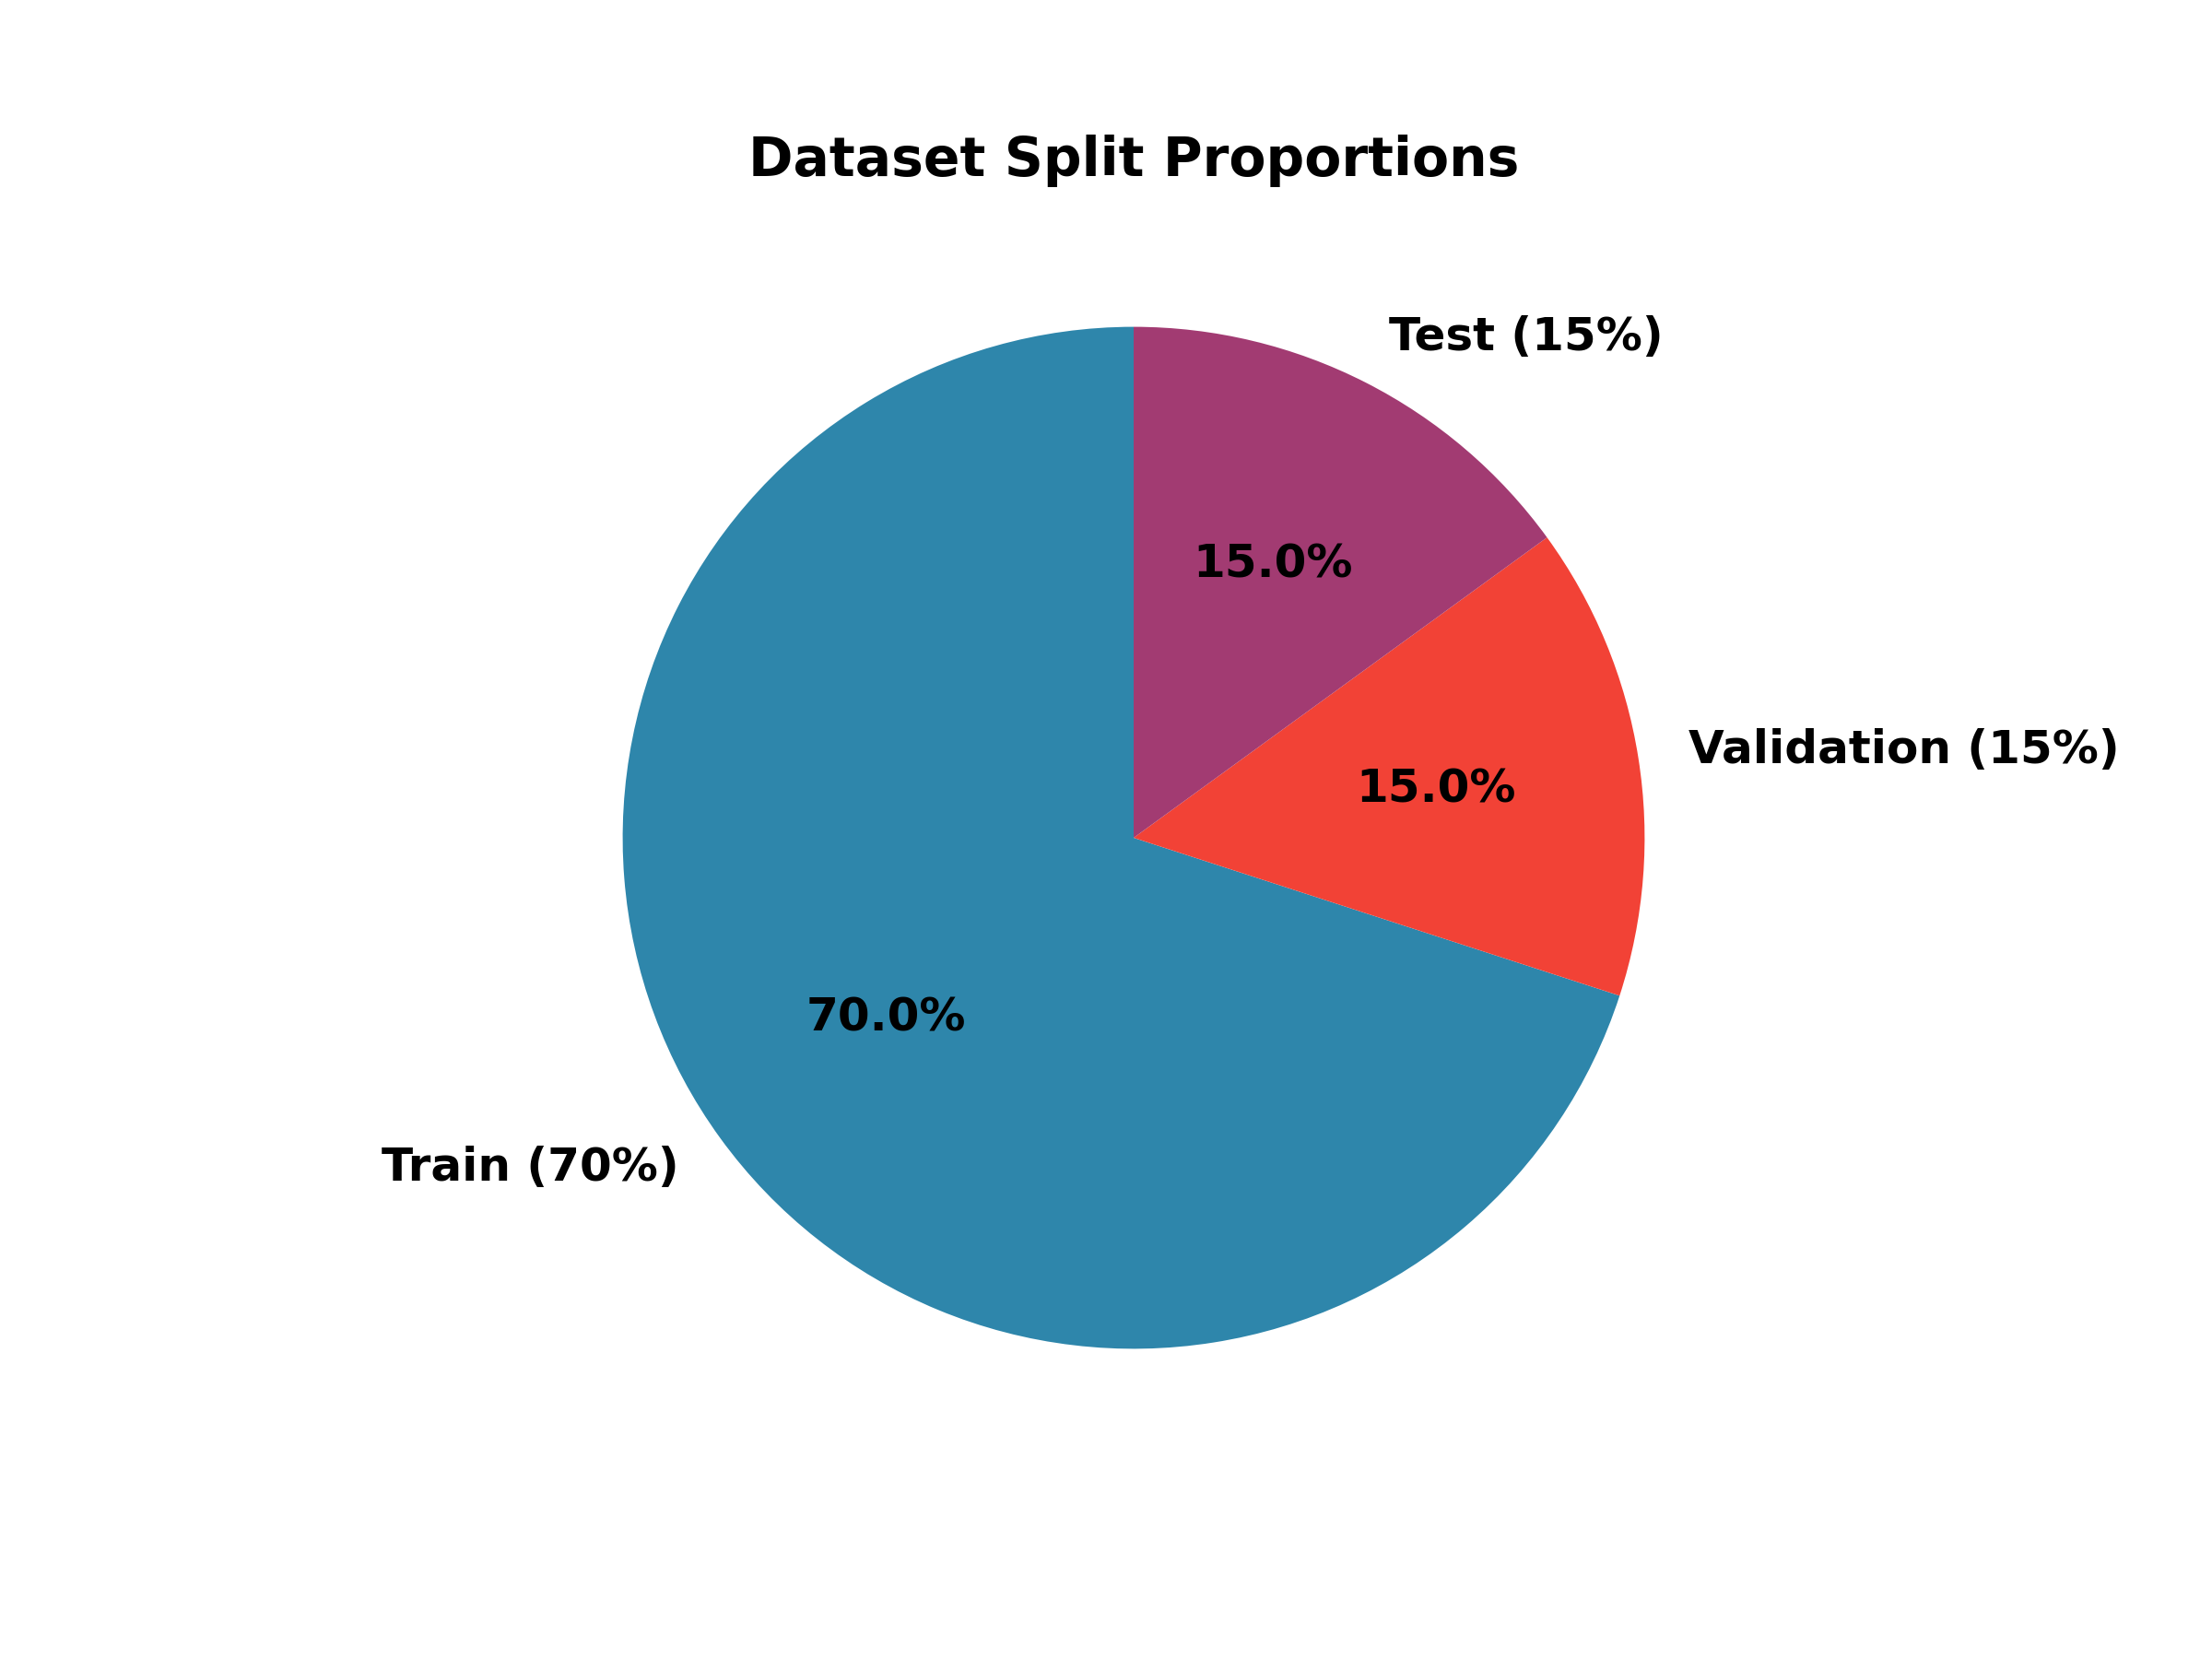
\includegraphics[width=0.48\textwidth]{images/dataset_split.png}
    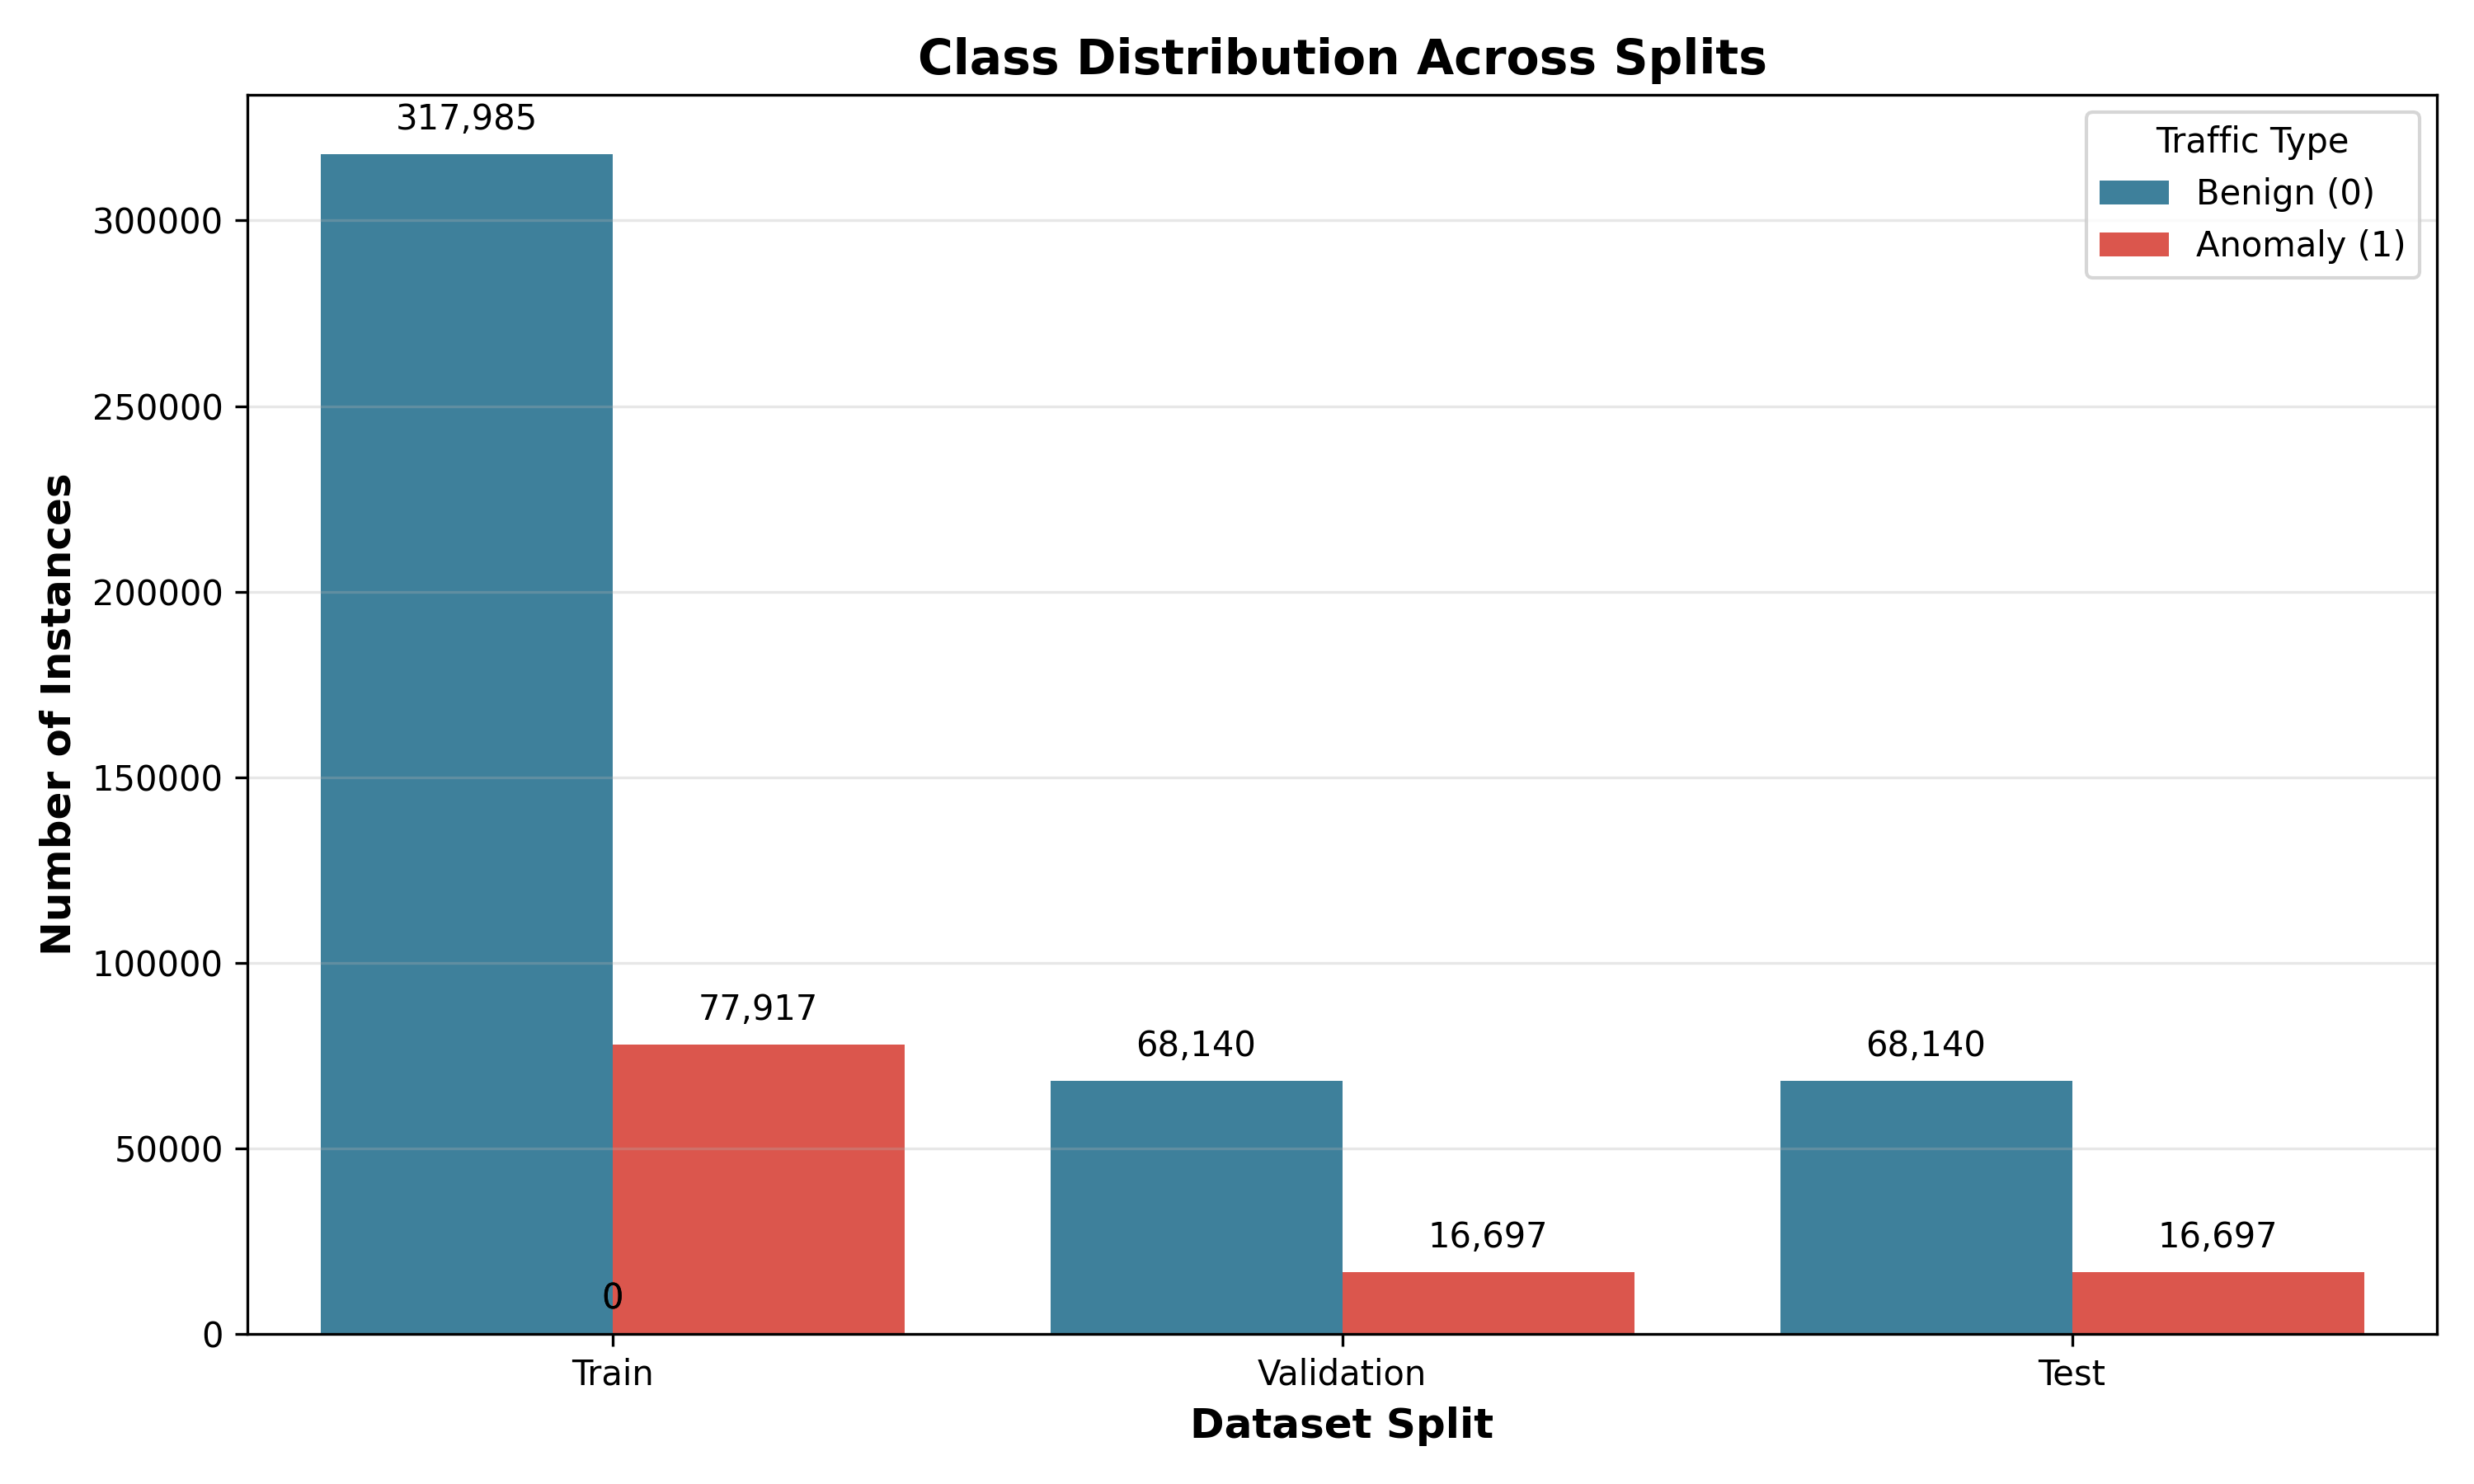
\includegraphics[width=0.48\textwidth]{images/class_distribution.png}
    \caption{Dataset split proportions and class distribution across subsets.}
    \label{fig:data_dist}
\end{figure}

\section{Data Preprocessing}

To construct the final input for the machine learning algorithms, an automated data processing pipeline was developed, consisting of the following sequential steps:

\begin{enumerate}
    \item \textbf{Data Cleaning:} We identified the presence of invalid structural values, including whitespace in column headers, and critical numerical anomalies. Specifically, `Infinity` values (arising from division by zero in bandwidth calculations like \texttt{Flow Bytes/s}) and `NaN` values were eliminated. As these affected less than 0.1\% of the dataset, direct removal (\textit{dropna}) was preferred over imputation to prevent the introduction of synthetic bias into the network behaviour distribution.
    \item \textbf{Dimensionality Reduction (Zero-Variance Check):} To mitigate computational noise, features demonstrating zero variance across the network captures were pruned. Eight features (e.g., \texttt{Bwd PSH Flags}, \texttt{Fwd Avg Bytes/Bulk}) were removed as they provide no discriminative power for distance-based detection mechanisms.
    \item \textbf{Stratified Sampling:} Given the massive size of the dataset ($>$1GB), loading the entire corpus triggered Out-Of-Memory (OOM) failures for algorithms with quadratic complexity ($\mathcal{O}(n^2)$). A 20\% stratified sampling was implemented, preserving the native 80/20 class imbalance while rendering the dataset computationally tractable ($\approx 565,000$ instances).
    \item \textbf{Data Split and Scaling:} The sample was split into 70\% Training, 15\% Validation, and 15\% Testing partitions. To ensure proper convergence of distance-based models and neural networks, attributes were scaled using \textit{StandardScaler}. To rigorously prevent data leakage, the scaler was fitted exclusively on the Training set and subsequently used to transform the Validation and Test sets.
\end{enumerate}

\section{AI Tools Acknowledgement}
During the development of this project, several Artificial Intelligence tools were utilized to support research, coding, and structuring:

\begin{itemize}
    \item \textbf{Gemini Pro:} Employed primarily for code review, debugging PyTorch tensor dimension mismatches during the Autoencoder implementation, and structuring Python data pipelines efficiently. It accelerated the resolution of Out-Of-Memory errors by suggesting optimal batch sizes and DataFrame chunking strategies.
    \item \textbf{Scite.ai / Elicit.com:} Used during the State of the Art literature review to track references and validate the relevance of classical vs. deep learning approaches in modern intrusion detection systems (IDS).
\end{itemize}
The rationale behind selecting these specific tools was their ability to trace verifiable sources and provide context-aware code optimizations without compromising the academic integrity of the experimental methodology.
